% Two paths from p to q in the punctured plane: the red path over the
% top and the blue path underneath can no longer be deformed into one
% another — a "meteor" (the deleted origin) is in the way.
% Source: book/tex/topology/top-more.tex (§ Homotopy and simply
% connected spaces) — second asy figure.
\documentclass[border=2mm]{standalone}
\usepackage{tikz}
\usepackage{amssymb}
\begin{document}
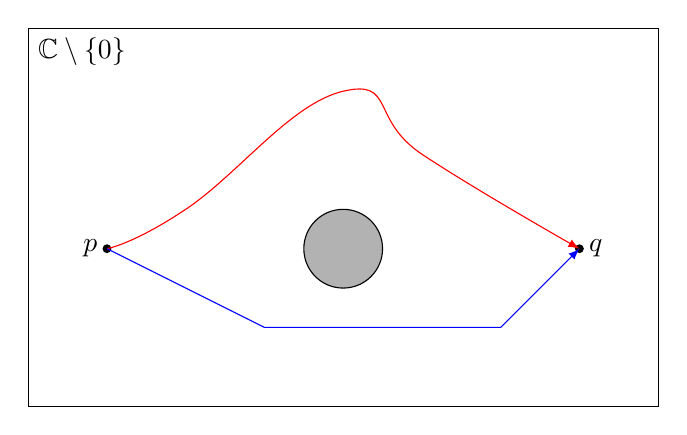
\begin{tikzpicture}[>=latex]
  % Bounding box standing in for the punctured plane.
  \draw (-4,-2) rectangle (4,2.8);
  \node[anchor=north west] at (-4,2.8) {$\mathbb{C} \setminus \{0\}$};
  % Endpoints.
  \fill (-3,0) circle (1.6pt) node[left] {$p$};
  \fill (3,0) circle (1.6pt) node[right] {$q$};
  % Red arc over the top.
  \draw[red,->] plot [smooth, tension=0.8]
    coordinates {(-3,0) (-2,0.5) (0,2) (1,1.2) (3,0)};
  % Blue polyline underneath.
  \draw[blue,->] (-3,0) -- (-1,-1) -- (2,-1) -- (3,0);
  % The meteor crater at the origin.
  \filldraw[fill=gray!60] (0,0) circle (0.5);
\end{tikzpicture}
\end{document}
